\section{Q-Learning}
\label{sec:qlearning_results}

\subsection{Design}
\label{sec:appendix_design}

\subsubsection{Constant Valuations}

Each bidder has a constant valuation $v_i=1.0$. Table~\ref{tab:exp1a_params} details the 10 factorial factors and fixed parameters. The $2^{10-1}$ Resolution~V half-fraction yields 512 cells, each replicated twice for 1{,}024 observations. The bid grid resolution is fixed at 11 discrete actions; a discretisation sensitivity analysis across grid sizes of 6, 11, and 21 is reported in Section~\ref{sec:appendix_robustness}.

\begin{table}[h]
\centering
\caption{Parameter settings for Experiment~1a (Constant Valuations).}
\label{tab:exp1a_params}
\begin{tabular}{l l l}
\toprule
\textbf{Factor} & \textbf{Low ($-1$)} & \textbf{High ($+1$)}\\
\midrule
Auction format & Second-price & First-price \\
Learning rate ($\alpha$) & 0.01 & 0.10 \\
Discount factor ($\gamma$) & 0.0 & 0.95 \\
Reserve price ($r$) & 0.0 & 0.5 \\
Initialisation & Zeros & Optimistic \\
Exploration & $\varepsilon$-greedy & Boltzmann \\
Update mode & Synchronous & Asynchronous \\
Number of bidders ($n$) & 2 & 4 \\
Information feedback & None (stateless) & Previous winning bid \\
Decay type & Linear & Exponential \\
\midrule
\multicolumn{3}{l}{\textbf{Fixed parameters}} \\
\midrule
Bid grid resolution & \multicolumn{2}{l}{11 discrete actions\footnotemark} \\
Number of episodes & \multicolumn{2}{l}{100{,}000} \\
\bottomrule
\end{tabular}
\footnotetext{Bid grid resolution is held constant at 11 levels. A discretisation sensitivity analysis varying the grid size is reported in Section~\ref{sec:appendix_robustness}.}
\end{table}

Experiment~1a compares $\varepsilon$-greedy and Boltzmann exploration using identical parameter schedules. Both decay from $1.0$ to $0.01$ over the first 90\% of training. To ensure comparability, Boltzmann exploration uses Q-range normalised temperatures, with the effective temperature $\tau_{\text{eff}} = \tau \cdot \max(\Delta Q, \epsilon)$ where $\Delta Q = \max_a Q(s,a) - \min_a Q(s,a)$ and $\epsilon = 10^{-8}$.\footnote{This normalisation ensures the softmax probabilities $\pi(a|s) \propto \exp(Q(s,a)/\tau_{\text{eff}})$ depend on the relative spacing of Q-values rather than their absolute scale, making the Boltzmann temperature comparable in effect to $\varepsilon$-greedy across different discount factors and training stages.} The decay type factor contrasts linear decay ($\varepsilon_t = 1 - t/t_{\max}$) with exponential decay ($\varepsilon_t = \varepsilon_0 \cdot (\varepsilon_{\min}/\varepsilon_0)^{t/t_{\max}}$); at the midpoint of training, exponential decay retains a higher exploration rate than linear decay (ratio approximately 1.6:1).\footnote{This asymmetry is by design. The factor tests whether front-loaded exploration (linear) or sustained exploration (exponential) better supports learning. The small estimated effect sizes across response variables confirm that decay shape is a secondary consideration relative to factors such as auction format and discount factor.}

\subsubsection{Affiliated Valuations}

Bidders receive private signals $s_i\in[0,1]$, and their valuations become interdependent through an affiliation parameter $\eta\in[0,1]$ via $v_i=(1-0.5\,\eta)\,s_i + 0.5\,\eta\,\bigl(\tfrac{1}{n-1}\sum_{j\neq i}s_j\bigr)$. Thus $\eta=0$ corresponds to purely private values and $\eta=1$ to strong common-value elements. Table~\ref{tab:exp1b_params} highlights the key parameters.

\begin{table}[h]
\centering
\caption{Parameter settings for Experiment~1b (Affiliated Valuations + Q-learning).}
\label{tab:exp1b_params}
\begin{tabular}{l l l}
\toprule
\textbf{Factor} & \textbf{Low ($-1$)} & \textbf{High ($+1$)}\\
\midrule
Auction format & Second-price & First-price \\
Number of bidders ($n$) & 2 & 4 \\
State information & Signal only & Signal + winner \\
\midrule
\textbf{Factor} & \multicolumn{2}{l}{\textbf{Levels}} \\
\midrule
Affiliation ($\eta$) & \multicolumn{2}{l}{0, 0.5, 1 (linear + quadratic contrasts)} \\
\midrule
\multicolumn{3}{l}{\textbf{Fixed parameters (from Experiment~1a results)}} \\
\midrule
Learning rate ($\alpha$) & \multicolumn{2}{l}{0.1} \\
Discount factor ($\gamma$) & \multicolumn{2}{l}{0.95} \\
Exploration & \multicolumn{2}{l}{$\varepsilon$-greedy} \\
Update mode & \multicolumn{2}{l}{Asynchronous} \\
Decay type & \multicolumn{2}{l}{Linear} \\
Reserve price ($r$) & \multicolumn{2}{l}{0.0} \\
Initialisation & \multicolumn{2}{l}{Zeros} \\
Bid grid resolution & \multicolumn{2}{l}{11 discrete actions} \\
Number of episodes & \multicolumn{2}{l}{100{,}000} \\
\bottomrule
\end{tabular}
\end{table}

\subsection{Constant Valuations (Experiment~1a)}
\label{sec:exp1a_results}

Experiment~1a deploys Q-learning agents with constant valuations ($v=1$) in a $2^{10-1}$ Resolution~V half-fraction spanning 10 factors and 1{,}024 observations. Under independent private values with constant valuations, revenue equivalence \citep{Vickrey1961} predicts identical expected revenue across auction formats. Despite this theoretical equivalence, average revenues in the final 1{,}000 episodes range from approximately 0.3 to 1.0, revealing substantial variability across configurations of learning parameters and market structure. The factorial analysis decomposes this variability into systematic effects attributable to individual factors and their interactions.

\begin{figure}[H]
  \centering
  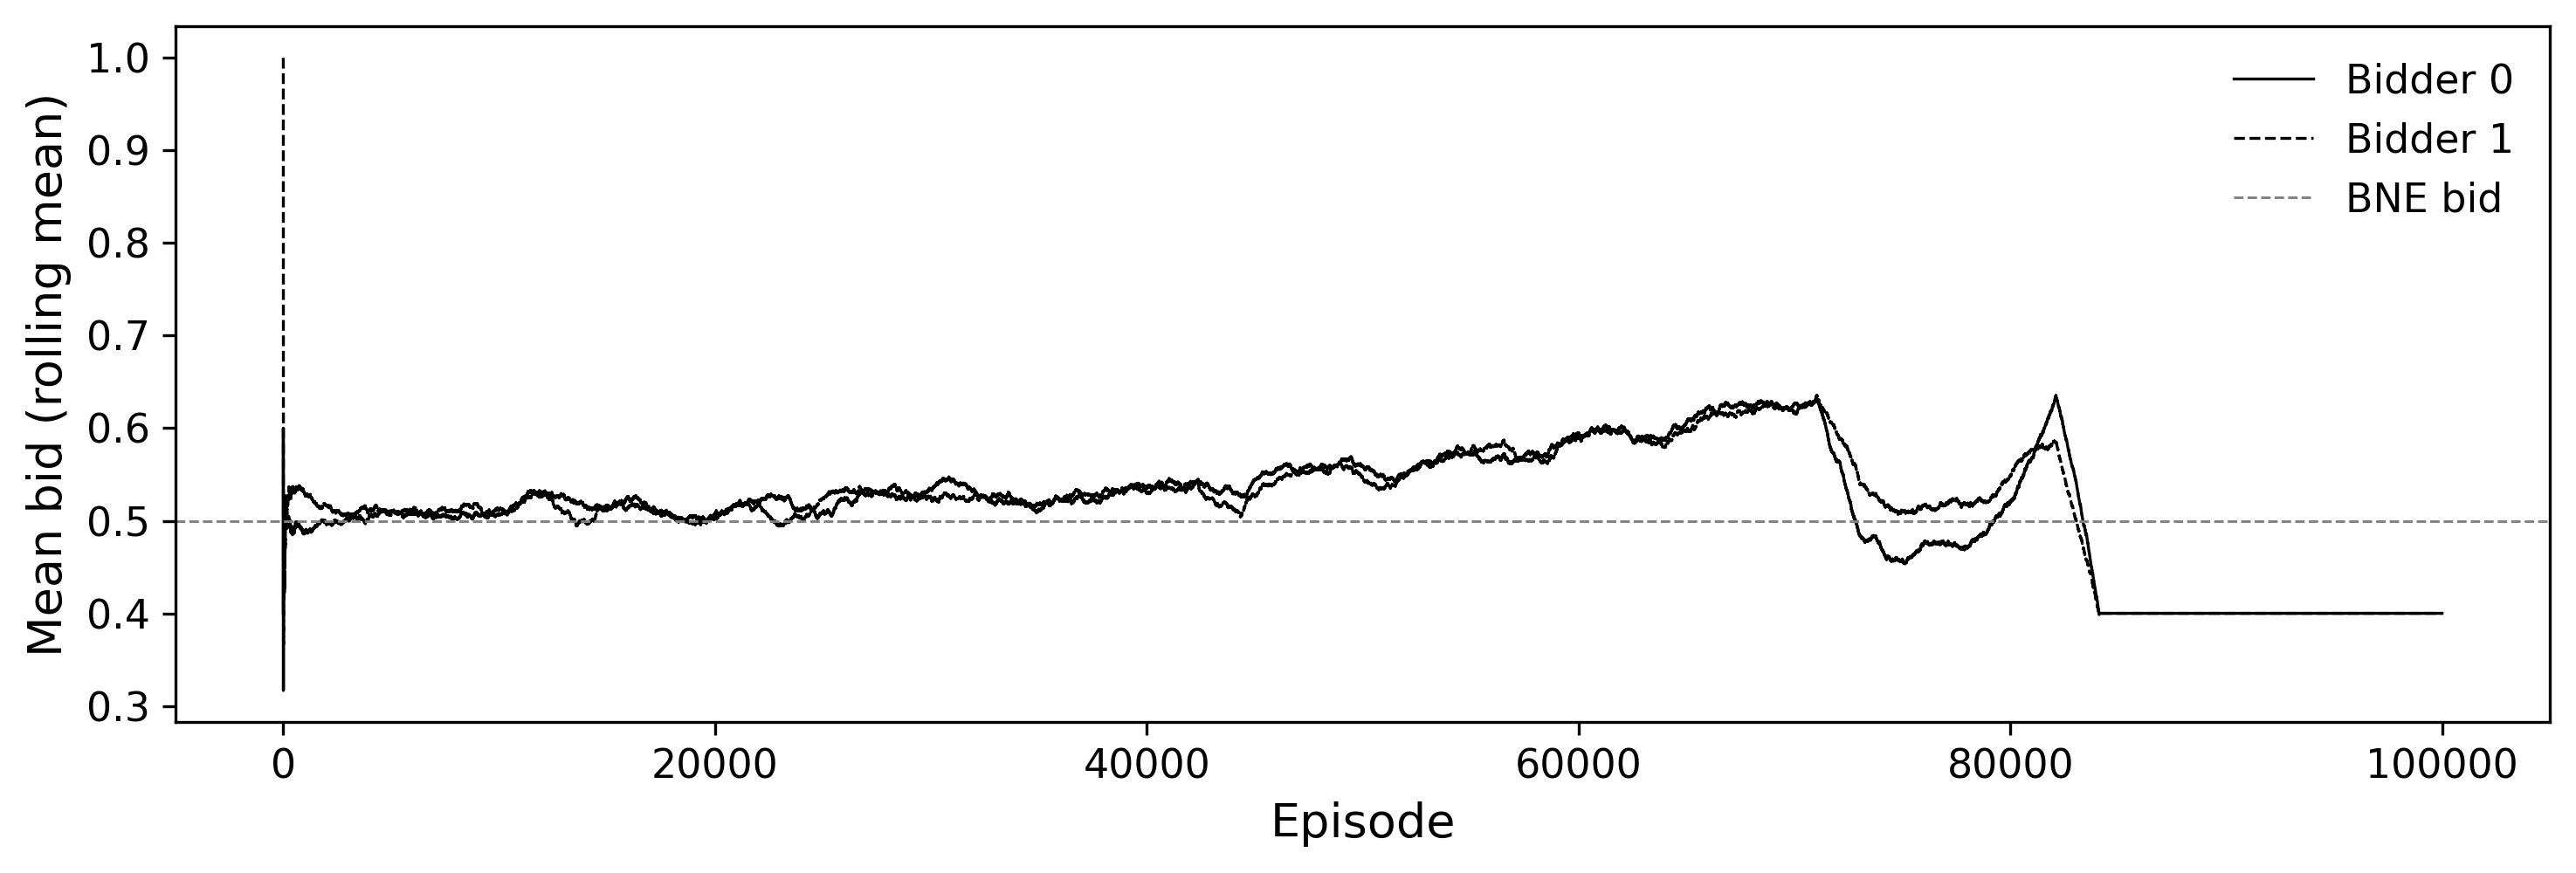
\includegraphics[width=\textwidth]{figures/e1a_trace}
  \caption{Representative learning trajectory for a single trial of Experiment~1a (first-price auction, 2~bidders, Boltzmann exploration, 10{,}000 episodes). Per-bidder mean bids (200-episode rolling mean) converge toward the BNE prediction over the course of training.}
  \label{fig:e1a_trace}
\end{figure}

\subsubsection{Revenue}

Number of bidders is the dominant factor for revenue ($|t| = \ExpOneARevFactorTOne$), followed by the discount factor $\gamma$ ($|t| = \ExpOneARevFactorTTwo$) and update mode ($|t| = \ExpOneARevFactorTThree$). Table~\ref{tab:exp1a_ranked_rev} ranks significant effects by absolute $t$-statistic. Moving from two to four bidders increases average revenue by \ExpOneARevTopPctEffect\% of the grand mean, an effect \ExpOneARevTopVsAuctionRatio{} times larger than that of auction format. Auction format, by contrast, does not exert a statistically significant main effect on revenue ($|t| = \ExpOneARevAuctionT$, $p \ExpOneARevAuctionPFmt$). First-price and second-price auctions produce nearly identical average revenues in the final 1{,}000 episodes (FPA mean \ExpOneARevMeanFPA{} vs.\ SPA mean \ExpOneARevMeanSPA). The main effects plot (Figure~\ref{fig:e1a_main_rev}) confirms these findings.

\begin{table}[H]
\centering
\caption{Experiment 1a: Significant effects for average revenue ($p < 0.05$), ranked by $|t|$.}
\label{tab:exp1a_ranked_rev}
\begin{tabular}{lrrl}
\toprule
\textbf{Effect} & \textbf{Coeff.} & \textbf{$|t|$} & \textbf{Direction} \\
\midrule
Number of bidders & 0.0871 & 17.75 & + \\
Discount factor ($\gamma$) & -0.0453 & 9.23 & $-$ \\
Update mode & 0.0366 & 7.45 & + \\
Discount factor ($\gamma$) $\times$ Number of bidders & 0.0298 & 6.09 & + \\
Auction format $\times$ Number of bidders & -0.0276 & 5.63 & $-$ \\
Reserve price & 0.0250 & 5.10 & + \\
Reserve price $\times$ Information feedback & -0.0219 & 4.47 & $-$ \\
Auction format $\times$ Discount factor ($\gamma$) & -0.0215 & 4.38 & $-$ \\
Auction format $\times$ Update mode & -0.0193 & 3.94 & $-$ \\
Information feedback & 0.0182 & 3.71 & + \\
\bottomrule
\end{tabular}
\end{table}


\begin{figure}[H]
  \centering
  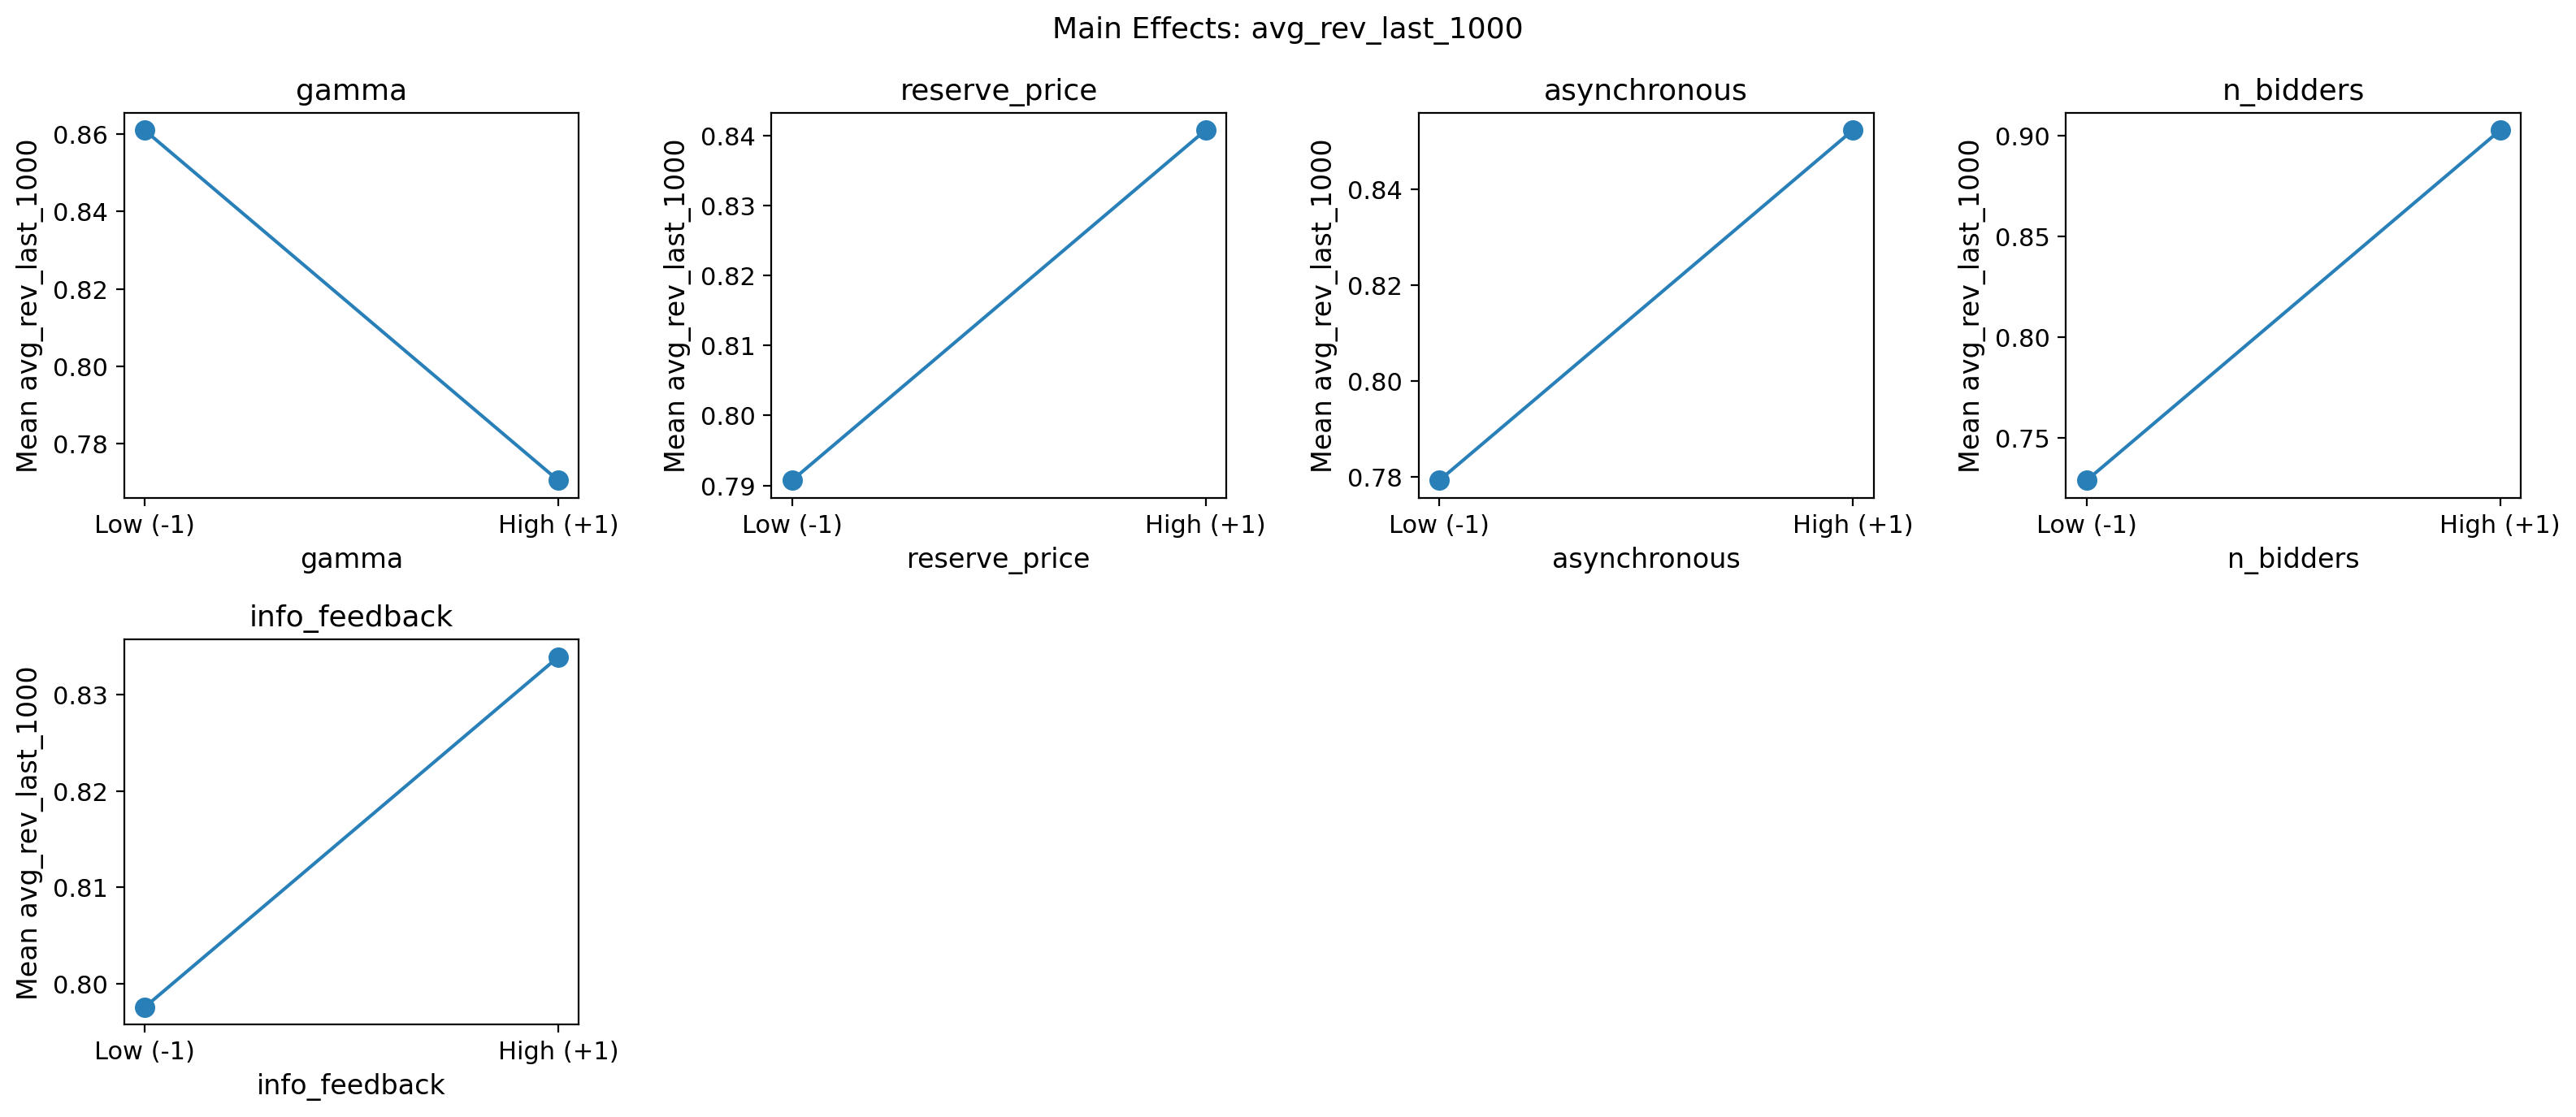
\includegraphics[width=0.7\textwidth]{figures/e1a_main_rev}
  \caption{Experiment~1a: Main effects plot for average revenue. Number of bidders and discount factor dominate; auction format has a negligible main effect.}
  \label{fig:e1a_main_rev}
\end{figure}

Although auction format has no significant main effect on final-episode revenue, it does interact significantly with other factors. The auction format $\times$ number of bidders interaction ($|t| = \ExpOneARevAuctionxNbidAbsT$) indicates that the format gap is larger in thin markets than in thick markets. The auction format $\times$ discount factor interaction ($|t| = \ExpOneARevAuctionxGammaAbsT$) shows that the auction format effect varies with the discount factor. Figure~\ref{fig:e1a_int_rev} displays these top interaction effects.

\begin{figure}[H]
  \centering
  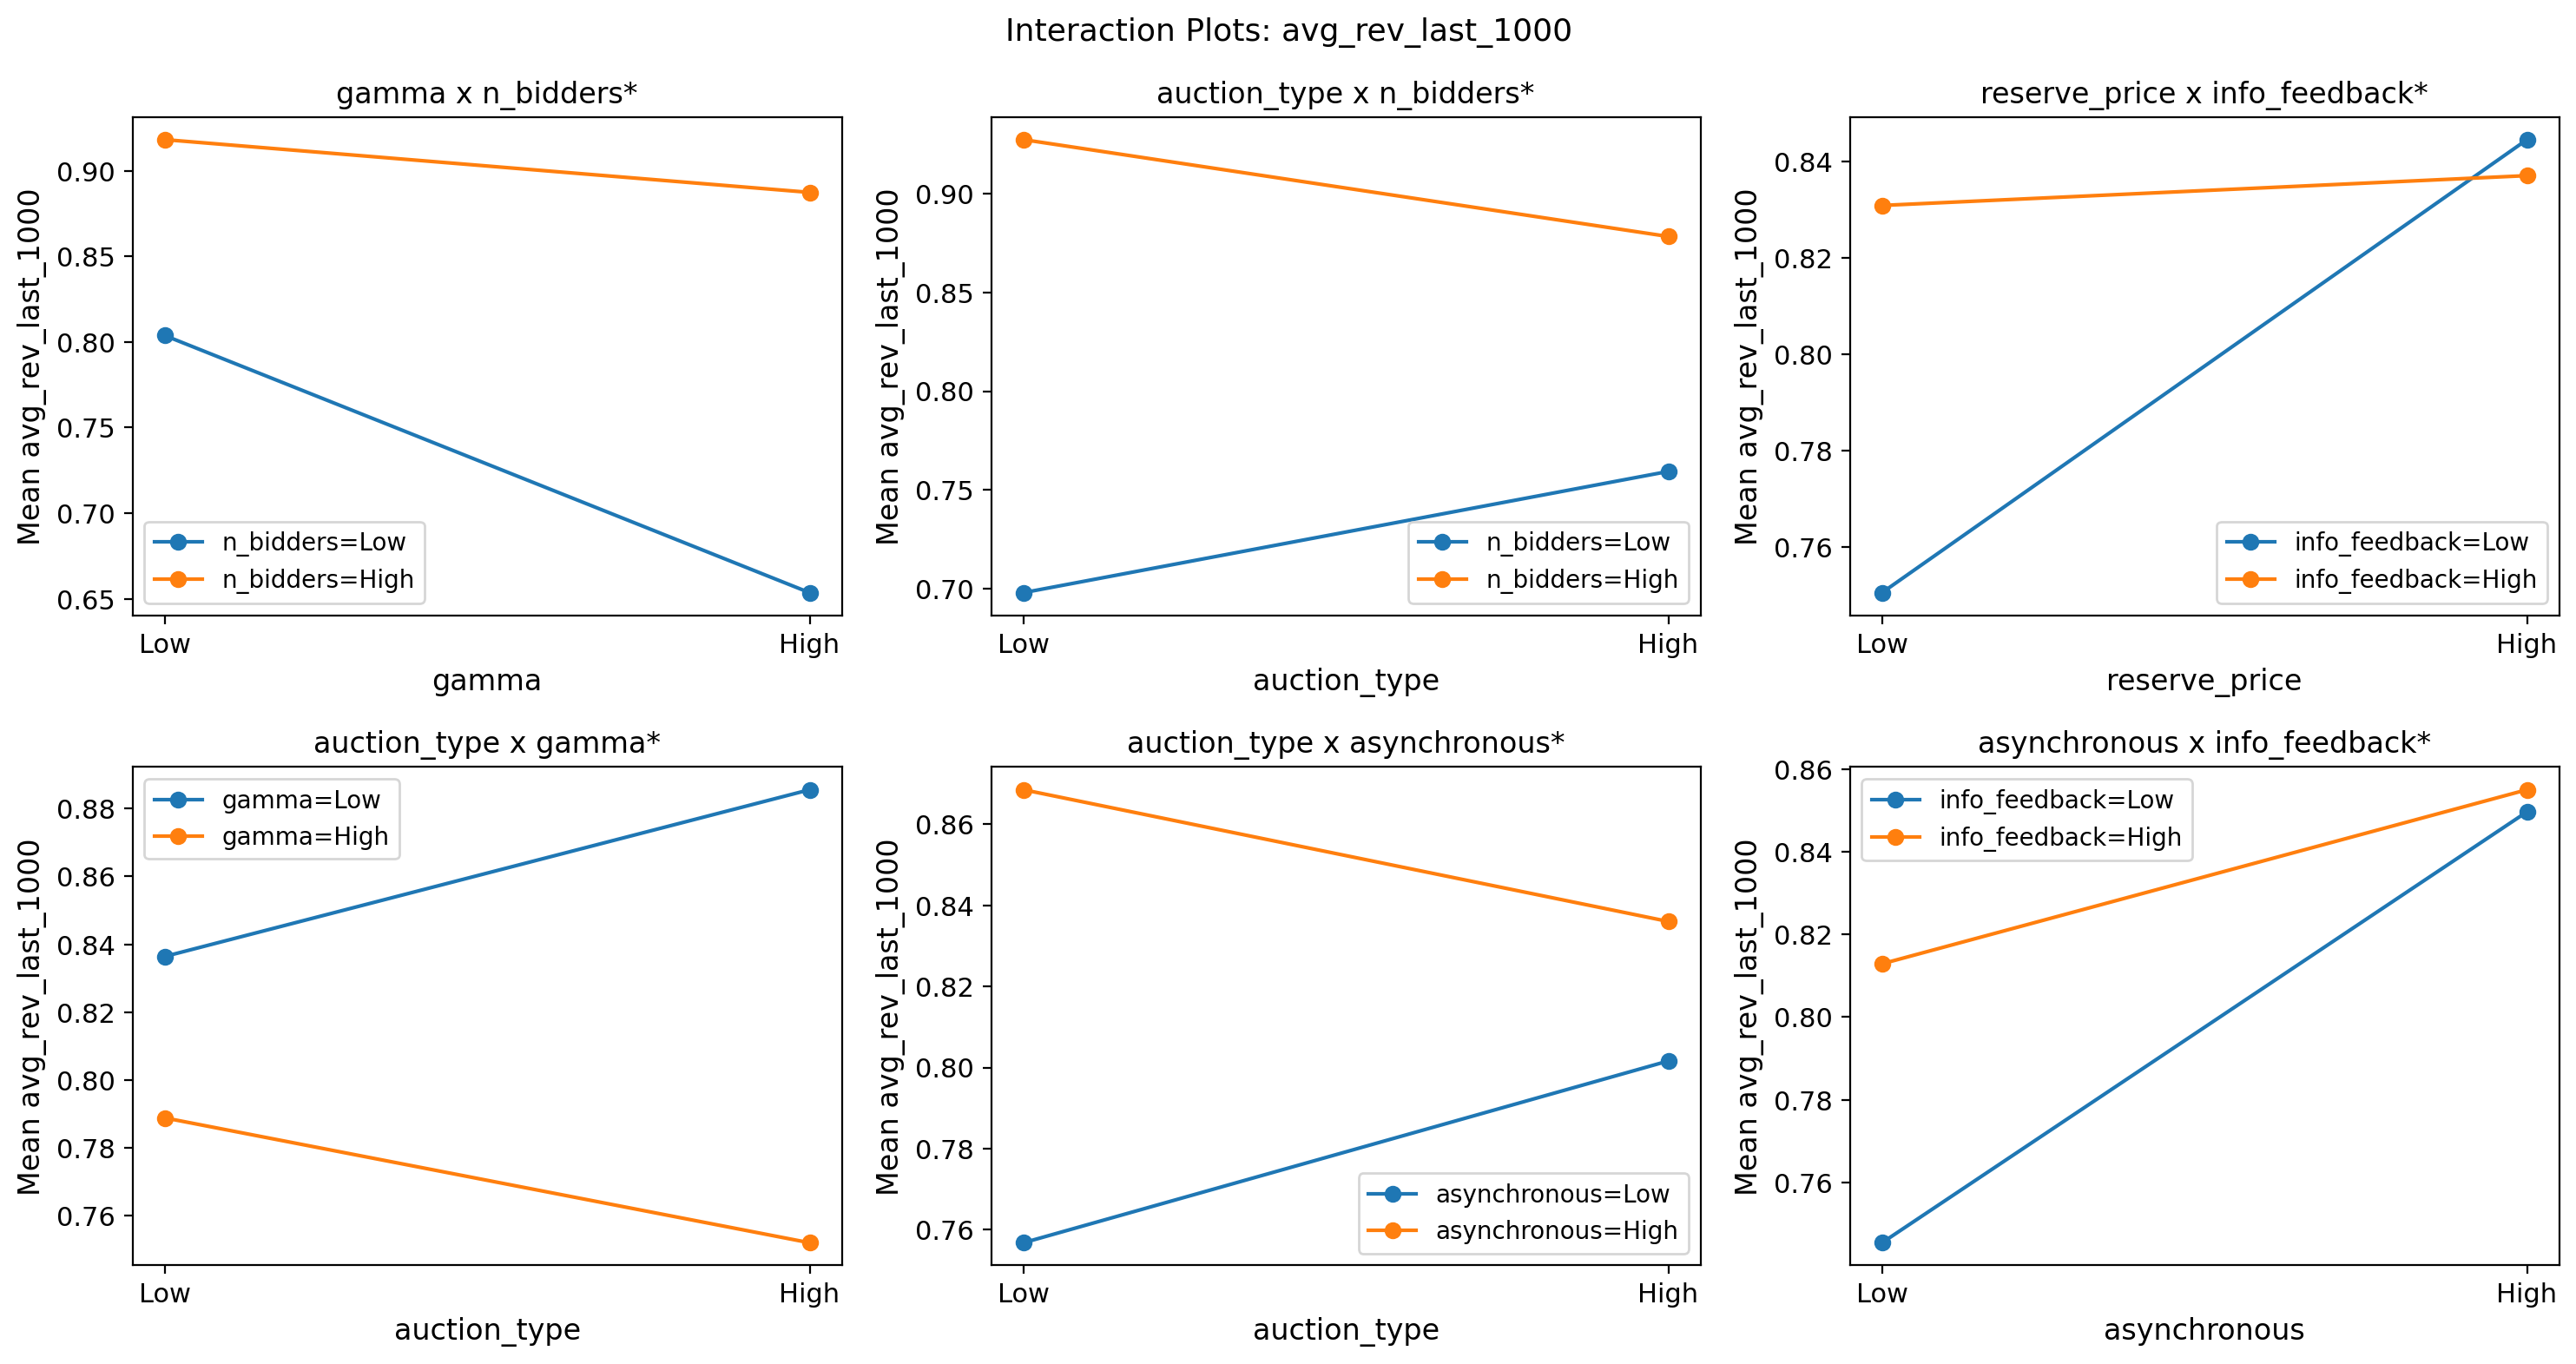
\includegraphics[width=0.7\textwidth]{figures/e1a_int_rev}
  \caption{Experiment~1a: Interaction plot for average revenue, showing the top two-way interactions. Non-parallel lines indicate that the effect of one factor depends on the level of another.}
  \label{fig:e1a_int_rev}
\end{figure}

\subsubsection{Price Volatility}

Table~\ref{tab:exp1a_ranked_vol} ranks the significant effects for price volatility. Market thickness, reserve price, discount factor, and update mode are the primary drivers (Figure~\ref{fig:e1a_main_vol}). Neither auction format nor exploration strategy has a significant direct effect.

\begin{table}[H]
\centering
\caption{Experiment 1a: Significant effects for price volatility ($p < 0.05$), ranked by $|t|$.}
\label{tab:exp1a_ranked_vol}
\begin{tabular}{lrrl}
\toprule
\textbf{Effect} & \textbf{Coeff.} & \textbf{$|t|$} & \textbf{Direction} \\
\midrule
Number of bidders & -0.0213 & 15.60 & $-$ \\
Reserve price & -0.0178 & 13.07 & $-$ \\
Discount factor ($\gamma$) & 0.0132 & 9.66 & + \\
Update mode & -0.0112 & 8.23 & $-$ \\
Reserve price $\times$ Update mode & 0.0069 & 5.08 & + \\
Exploration strategy $\times$ Information feedback & -0.0059 & 4.30 & $-$ \\
Initialisation & 0.0059 & 4.30 & + \\
Reserve price $\times$ Number of bidders & 0.0053 & 3.89 & + \\
Number of bidders $\times$ Information feedback & -0.0051 & 3.71 & $-$ \\
Discount factor ($\gamma$) $\times$ Reserve price & -0.0042 & 3.11 & $-$ \\
\bottomrule
\end{tabular}
\end{table}


\begin{figure}[H]
  \centering
  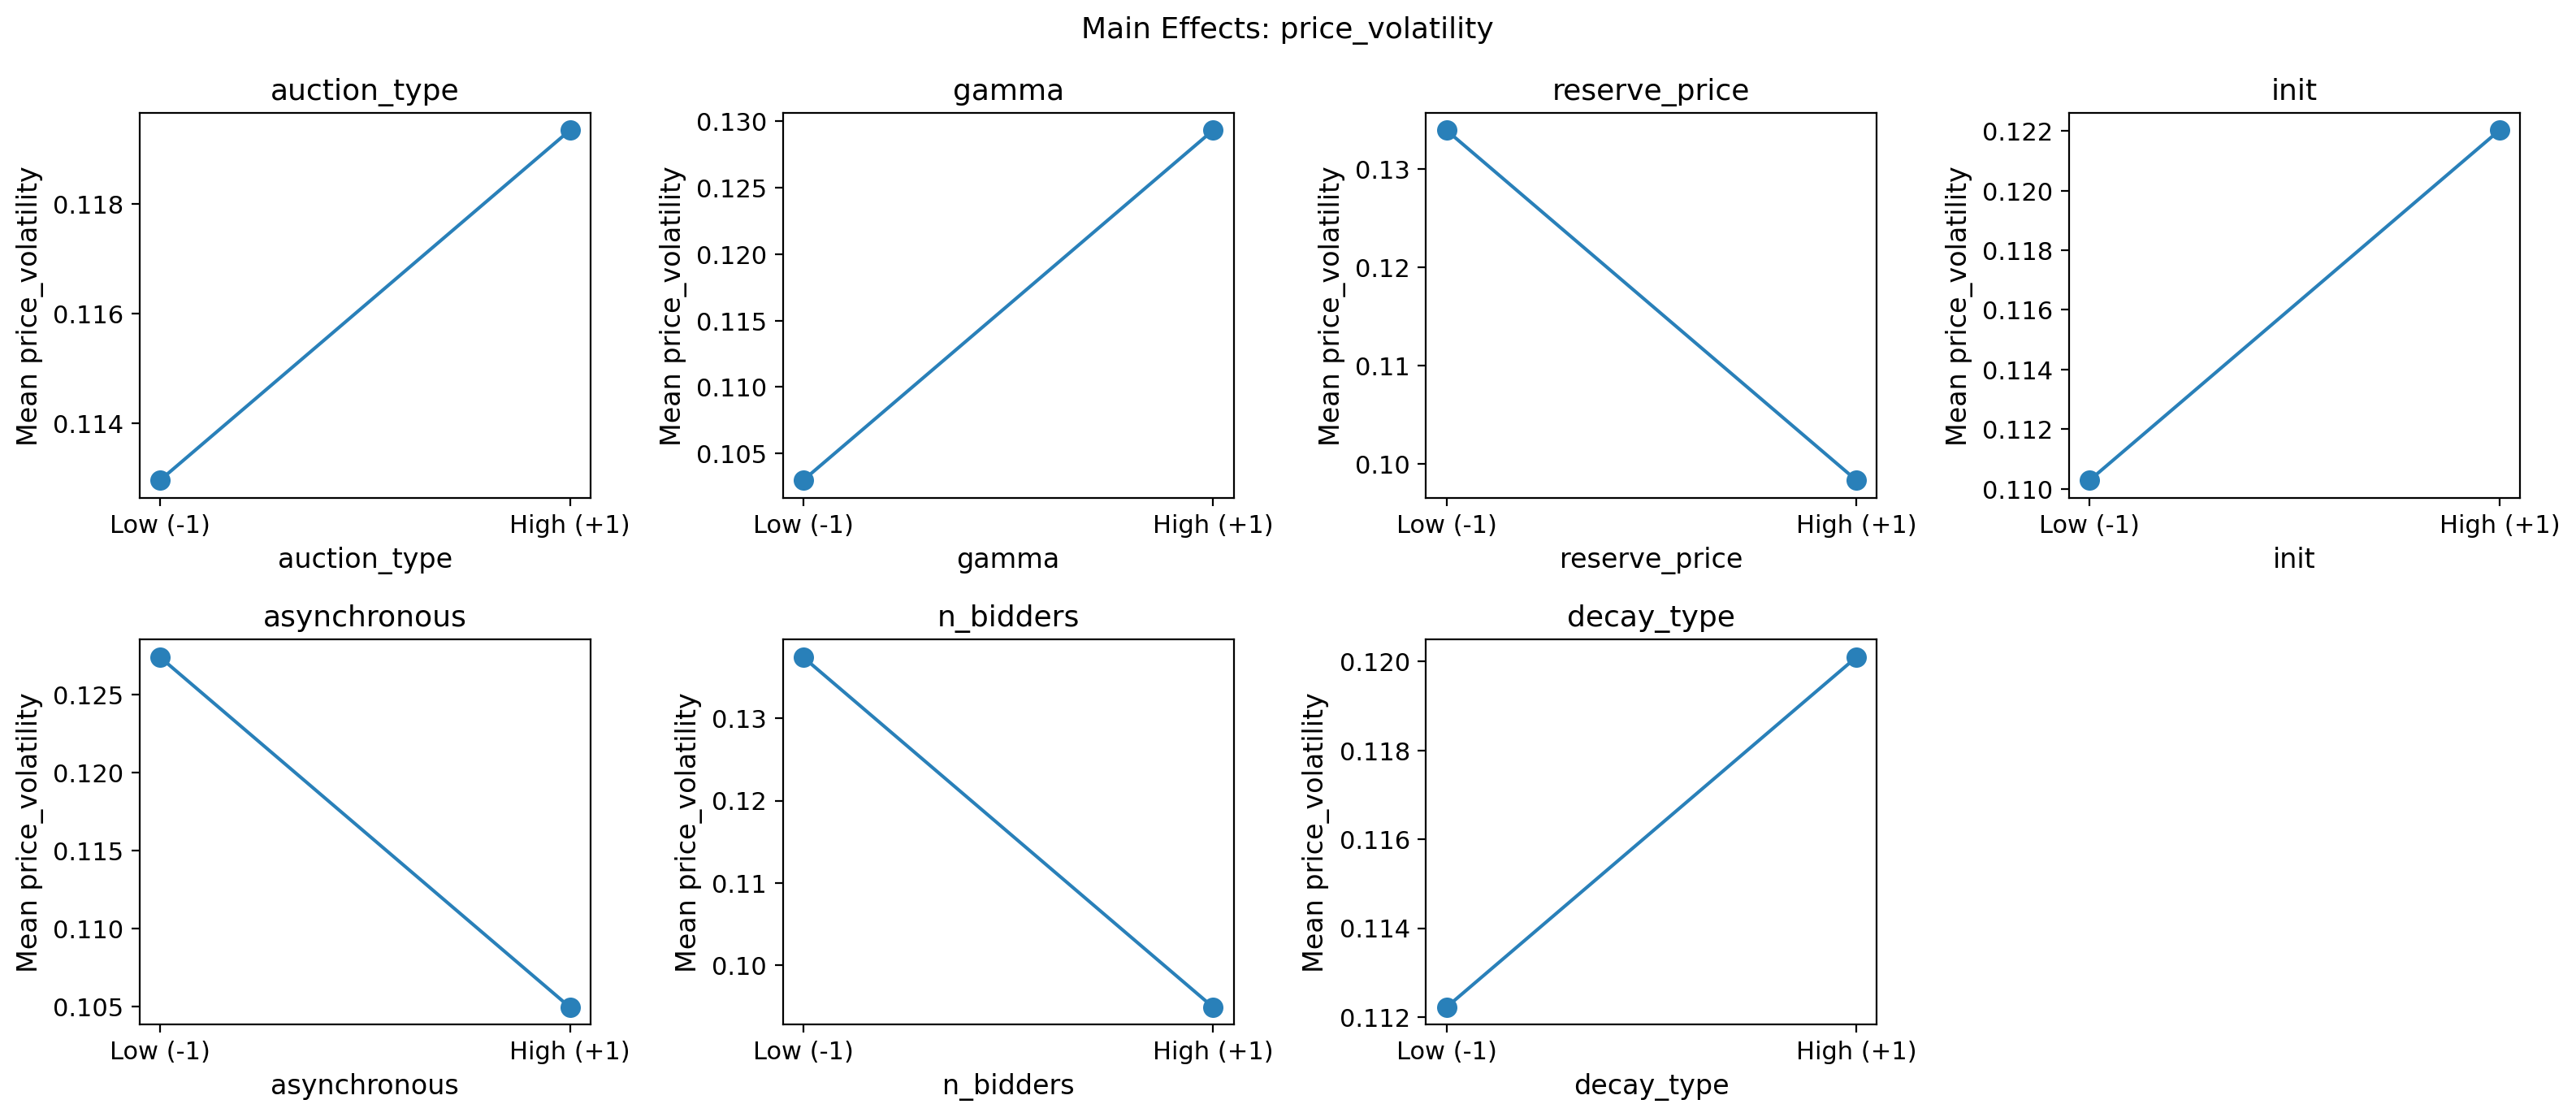
\includegraphics[width=0.7\textwidth]{figures/e1a_main_vol}
  \caption{Experiment~1a: Main effects plot for price volatility. Number of bidders, reserve price, and discount factor are the primary drivers.}
  \label{fig:e1a_main_vol}
\end{figure}

Model adequacy diagnostics confirm these findings (Appendix~\ref{sec:appendix_robustness}).

\subsection{Affiliated Valuations (Experiment~1b)}
\label{sec:exp1b_results}

Experiment~1b generalises the framework to affiliated valuations with $\eta \in \{0, 0.5, 1\}$, testing whether the revenue ranking predicted by \citet{MilgromWeber1982} (SPA $\geq$ FPA under affiliation) emerges under Q-learning. The $3 \times 2^3 = 24$ mixed-level factorial crosses auction format, affiliation strength, number of bidders, and state information, with hyperparameters fixed at levels identified in Experiment~1a.

\begin{figure}[H]
  \centering
  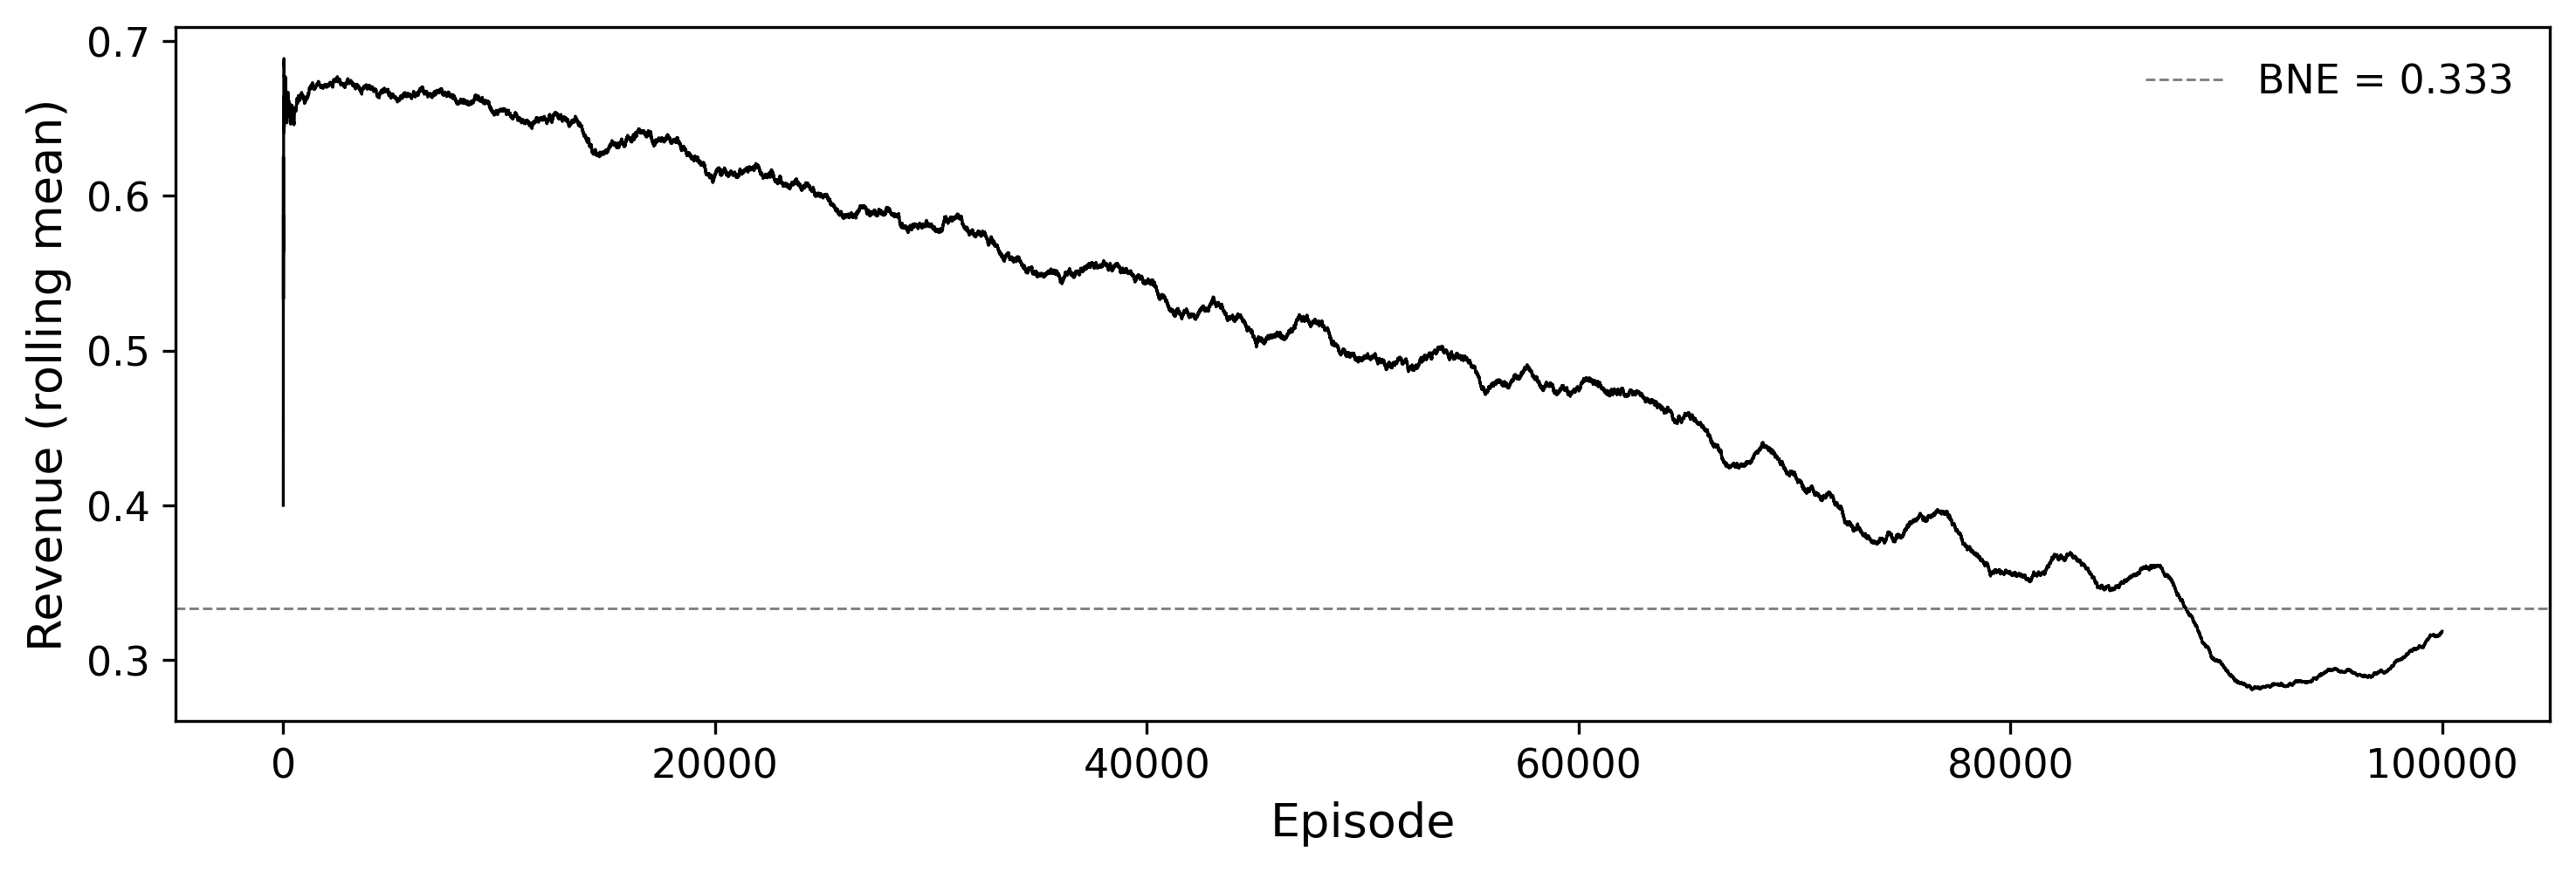
\includegraphics[width=\textwidth]{figures/e1b_trace}
  \caption{Representative learning trajectory for a single trial of Experiment~1b (first-price auction, $\eta = 0.5$, 2~bidders, 10{,}000 episodes). Rolling-mean revenue converges near the BNE prediction.}
  \label{fig:e1b_trace}
\end{figure}

\subsubsection{Revenue}

Number of bidders is the dominant factor for revenue ($|t| = \ExpOneBRevNbidAbsT$), with the low-to-high shift increasing revenue by \ExpOneBRevTopPctEffect\% of the grand mean. Auction format is statistically significant but economically modest ($|t| = \ExpOneBRevAuctionT$, $p \ExpOneBRevAuctionPFmt$). Table~\ref{tab:exp1b_ranked_rev} reports the full effect hierarchy; Figure~\ref{fig:e1b_main_rev} displays the directional patterns.

\begin{table}[H]
\centering
\caption[Experiment 1b: significant effects for average revenue ($p < 0.05$), ranked by $|t|$]{\textbf{Experiment 1b: significant effects for average revenue ($p < 0.05$), ranked by $|t|$.}}
\label{tab:exp1b_ranked_rev}
\begin{tabular}{lrrl}
\toprule
\textbf{Effect} & \textbf{Coeff.} & \textbf{$|t|$} & \textbf{Direction} \\
\midrule
Number of bidders & 0.0552 & 6.53 & + \\
State information & -0.0495 & 5.85 & $-$ \\
Auction format $\times$ Number of bidders & -0.0285 & 3.38 & $-$ \\
Auction format & -0.0268 & 3.17 & $-$ \\
Number of bidders $\times$ State information & -0.0263 & 3.11 & $-$ \\
\bottomrule
\end{tabular}
\end{table}


\begin{figure}[H]
  \centering
  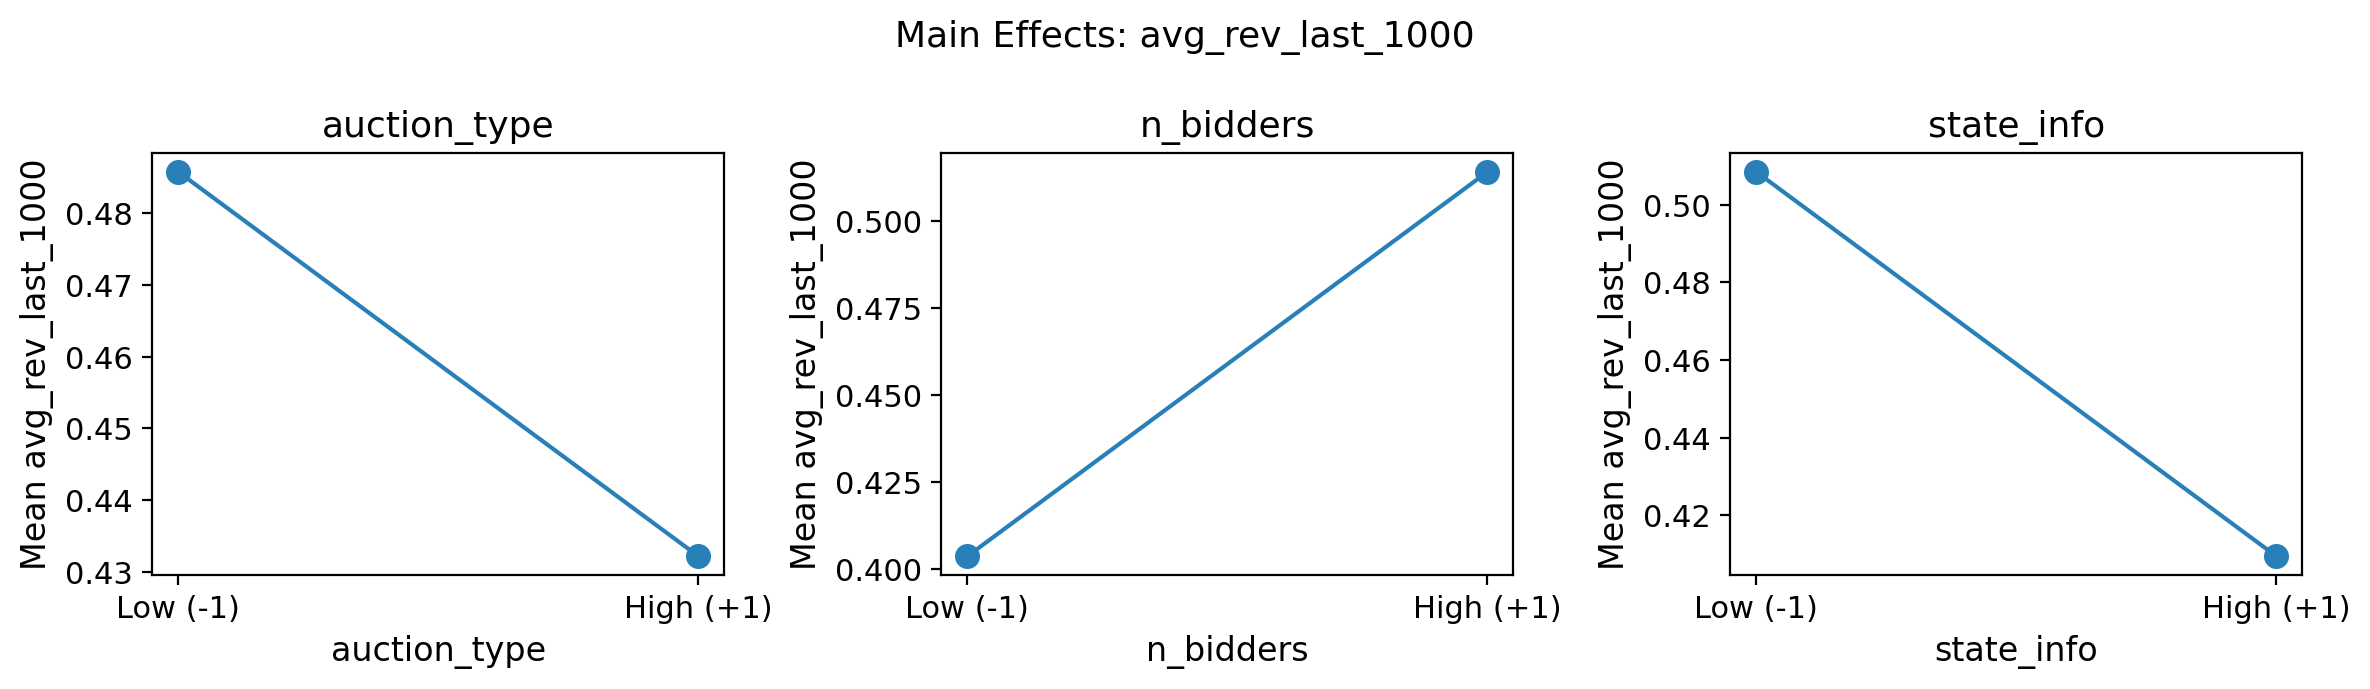
\includegraphics[width=0.7\textwidth]{figures/e1b_main_rev}
  \caption{Experiment~1b: Main effects plot for average revenue. First-price auctions reduce revenue across all factor configurations.}
  \label{fig:e1b_main_rev}
\end{figure}

The affiliation parameter $\eta$ has no significant effect on any primary outcome, despite spanning the full range from independent private values to near-common values. This null result contrasts with the \citet{MilgromWeber1982} prediction that affiliation should increase revenue under second-price rules. The number of bidders moderates the auction type effect, with the first-price revenue penalty smaller under four bidders than under two. State information also influences revenue outcomes. The interaction plot (Figure~\ref{fig:e1b_int_rev}) displays these moderating relationships.

\begin{figure}[H]
  \centering
  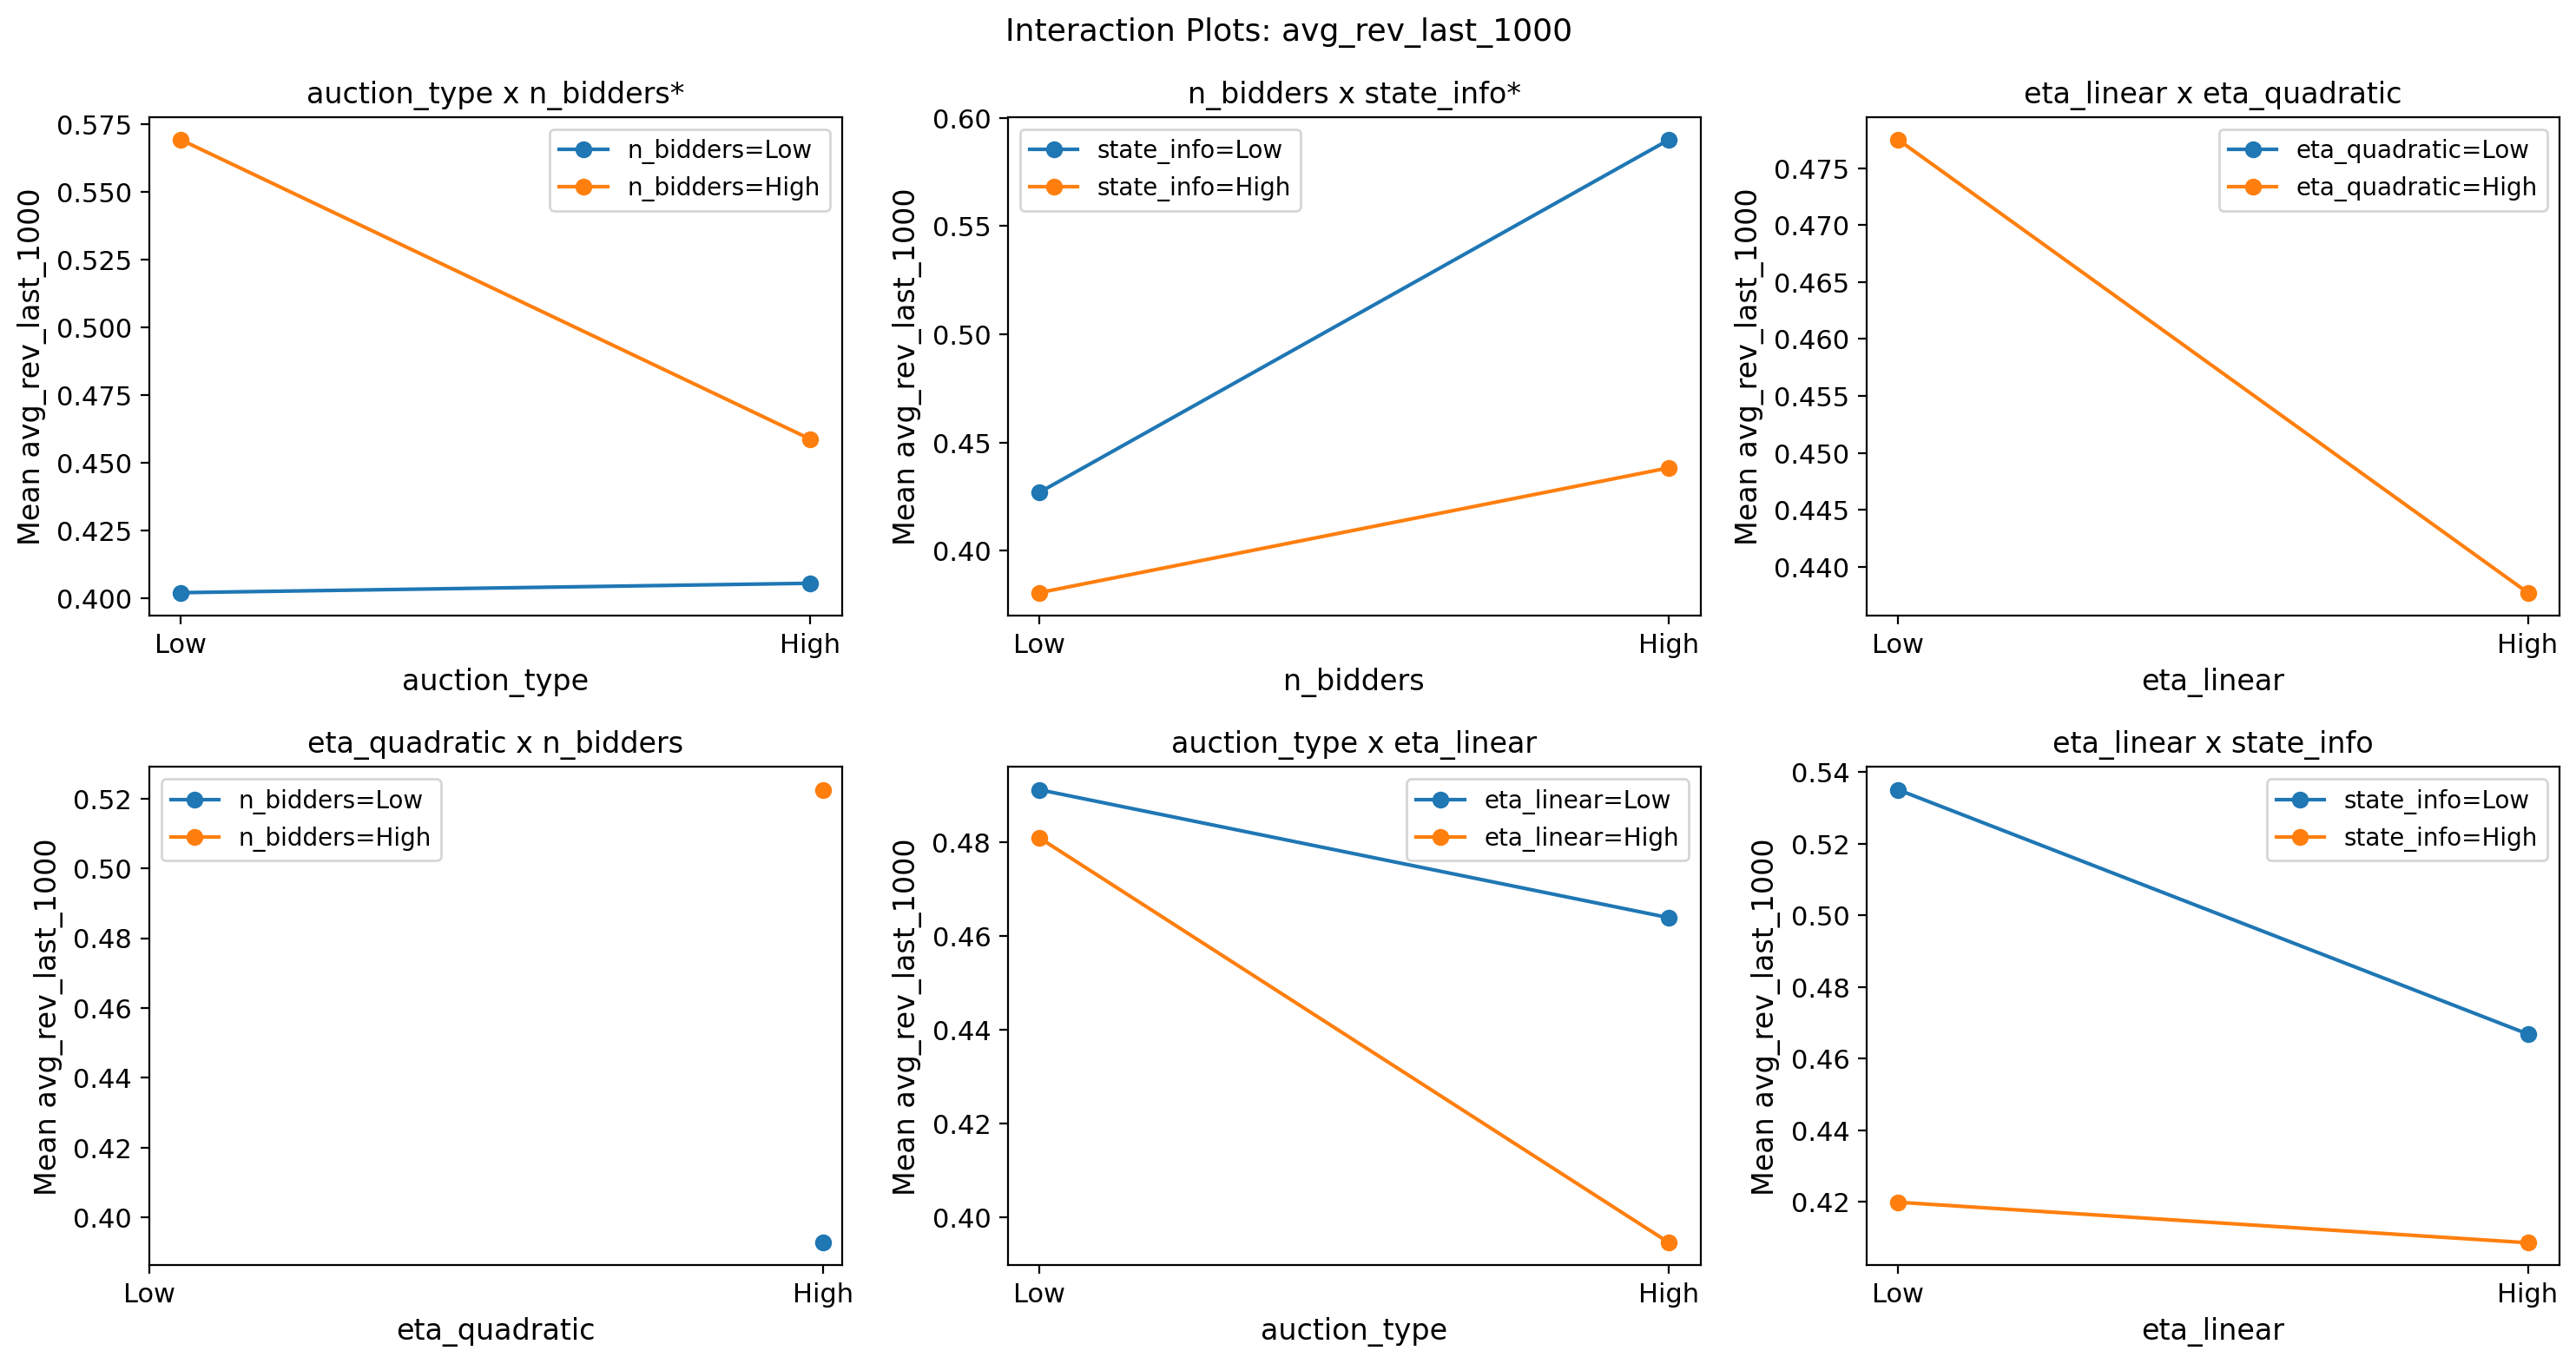
\includegraphics[width=0.7\textwidth]{figures/e1b_int_rev}
  \caption{Experiment~1b: Interaction plot for average revenue. The auction type $\times$ number of bidders and auction type $\times$ state information interactions are among the strongest two-way effects.}
  \label{fig:e1b_int_rev}
\end{figure}

End-state revenue (final 1{,}000 episodes) and lifetime revenue (all episodes) reveal different patterns across auction formats. Both formats generate higher revenue during the learning phase than at convergence. First-price auctions show a learning-phase premium roughly three times larger than second-price, which offsets the end-state revenue gap.\footnote{First-price auctions show a learning-phase premium of \ExpOneBFPAPremium{} (mean lifetime revenue \ExpOneBAllMeanFPA{} vs.\ end-state \ExpOneBEndMeanFPA), while second-price auctions show a premium of \ExpOneBSPAPremium{} (\ExpOneBAllMeanSPA{} vs.\ \ExpOneBEndMeanSPA).} In the factorial model for lifetime revenue, the number of bidders and state information remain significant, but auction format is no longer significant, rendering the two formats statistically indistinguishable over the full trajectory.\footnote{Lifetime revenue model: $R^2 = \ExpOneBAllRevRsq$; number of bidders $|t| = \ExpOneBAllRevNbidAbsT$, state information $|t| = \ExpOneBAllRevStateAbsT$, auction format $|t| = \ExpOneBAllRevAuctionAbsT$ ($p \ExpOneBAllRevAuctionPFmt$).} The auction format $\times$ number of bidders interaction persists for lifetime revenue. With two bidders, first-price auctions generate higher lifetime revenue, while with four bidders, second-price auctions lead.\footnote{Interaction: $|t| = \ExpOneBAllRevAuctionxNbidAbsT$, $p \ExpOneBAllRevAuctionxNbidPFmt$. Two bidders: FPA \ExpOneBAllFPATwoBid{} vs.\ SPA \ExpOneBAllSPATwoBid; four bidders: SPA \ExpOneBAllSPAFourBid{} vs.\ FPA \ExpOneBAllFPAFourBid.}

\subsubsection{Price Volatility}

Unlike Experiment~1a, where auction type had minimal effect on volatility, first-price auctions now significantly raise price volatility under affiliated valuations. Table~\ref{tab:exp1b_ranked_vol} shows auction type among the significant effects for volatility. The main effects plot (Figure~\ref{fig:e1b_main_vol}) confirms the directional increase. The number of bidders and affiliation strength also contribute to volatility differences across configurations.

\begin{table}[H]
\centering
\caption{Experiment 1b: Significant effects for price volatility ($p < 0.05$), ranked by $|t|$.}
\label{tab:exp1b_ranked_vol}
\begin{tabular}{lrrl}
\toprule
\textbf{Effect} & \textbf{Coeff.} & \textbf{$|t|$} & \textbf{Direction} \\
\midrule
Number of bidders & -0.0147 & 6.15 & $-$ \\
State information & 0.0124 & 5.22 & + \\
Auction format & 0.0090 & 3.77 & + \\
Auction format $\times$ Affiliation (linear) & 0.0074 & 2.54 & + \\
Auction format $\times$ Number of bidders & 0.0056 & 2.34 & + \\
\bottomrule
\end{tabular}
\end{table}


\begin{figure}[H]
  \centering
  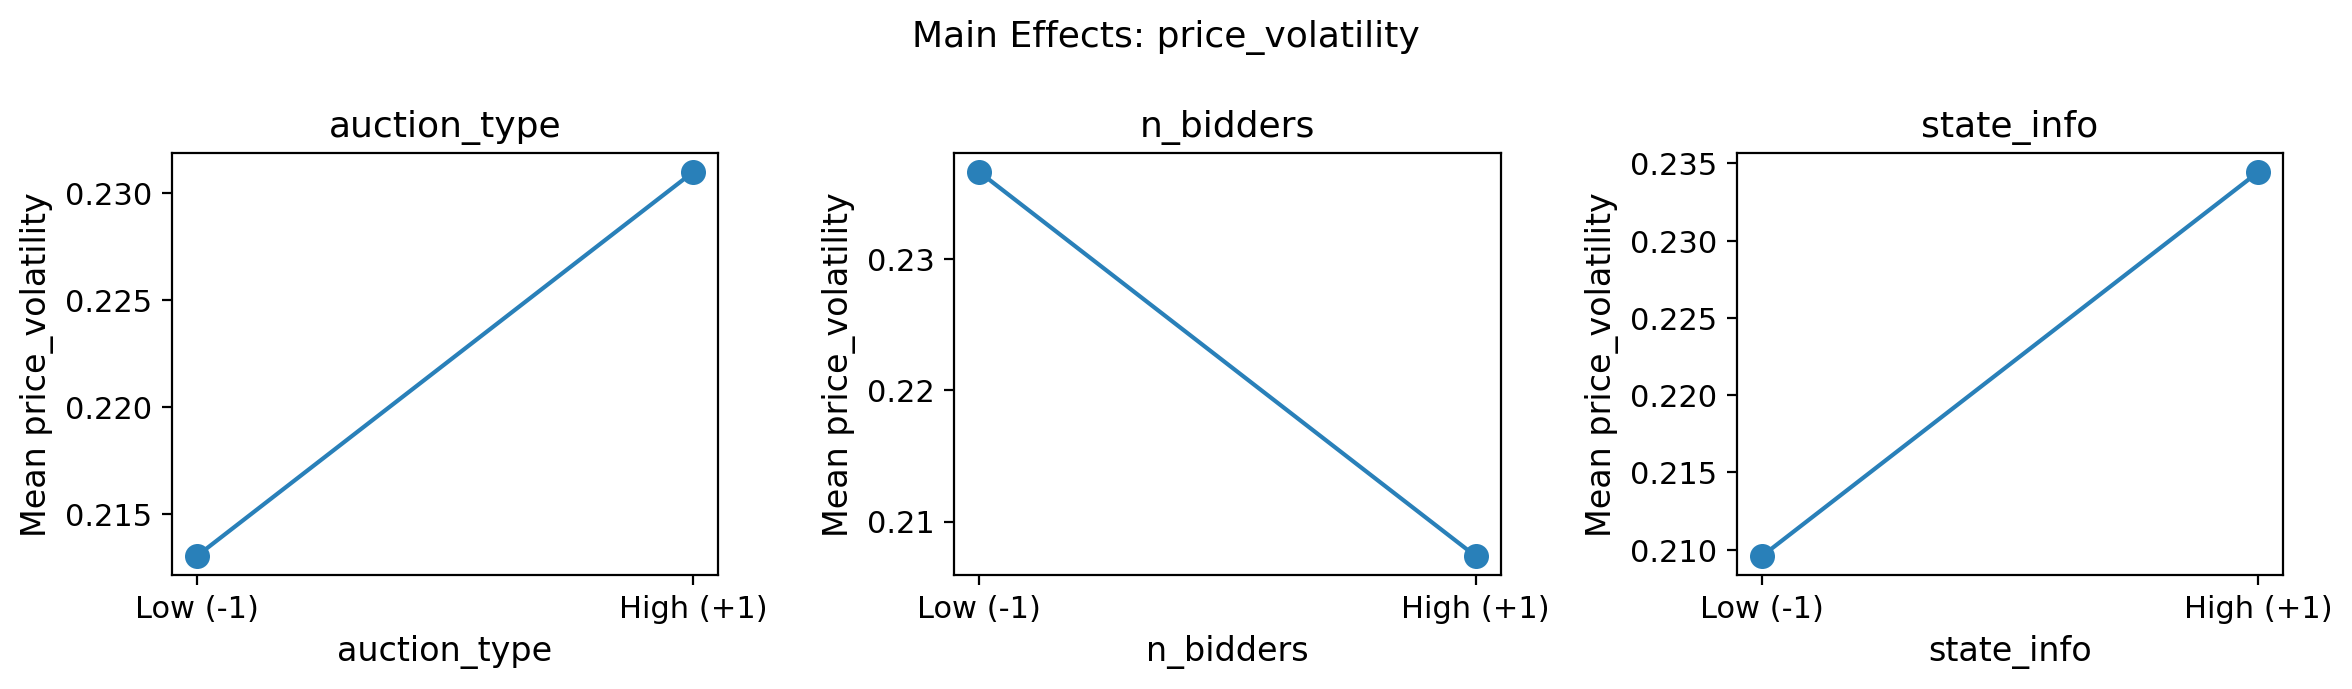
\includegraphics[width=0.7\textwidth]{figures/e1b_main_vol}
  \caption{Experiment~1b: Main effects plot for price volatility.}
  \label{fig:e1b_main_vol}
\end{figure}

Model adequacy diagnostics confirm these findings (Appendix~\ref{sec:appendix_robustness}).

\subsection{Sensitivity Analysis}
\label{sec:qlearning_sensitivity}

Global sensitivity analysis independently confirms the factorial rankings. In Experiment~1a, the number of bidders achieves the highest total-order Sobol' index for revenue ($S_T = 0.24$) and dominates four of five responses, while reserve price dominates the no-sale rate ($S_T = 0.27$). Learning rate and initialisation are negligible across all responses. Cross-method concordance is high (mean Spearman $\rho = 0.87$), confirming stable factor rankings across all seven methods. In Experiment~1b, the number of bidders again dominates revenue ($S_T = 0.22$), while auction format is the most important factor for winner's curse frequency ($S_T = 0.36$). The affiliation parameter $\eta$ overwhelmingly drives signal responsiveness ($S_T = 0.40$), confirming that the experimental manipulation successfully modulates bidding behaviour. Cross-method concordance is low ($\rho = 0.33$), reflecting the small design (24 cells). Detailed per-factor Sobol' indices appear in Appendix~\ref{sec:appendix_sensitivity_tables} (Tables~\ref{tab:sens_exp1a}--\ref{tab:sens_exp1b_b}).

\subsection{Summary}

The number of bidders is the strongest determinant of seller outcomes across both Q-learning experiments. In Experiment~1a, it is followed by the discount factor and update mode, while auction format does not significantly affect end-state revenue but interacts with competitive pressure and temporal discounting. This null result for auction format provides a baseline; subsequent experiments show that the importance of format is context-dependent, emerging under affiliated valuations and budget-constrained pacing. Price volatility in Experiment~1a is governed by market thickness, reserve prices, and the discount factor.

In Experiment~1b, the number of bidders dominates all other factors ($|t| = \ExpOneBRevNbidAbsT$). Auction format reduces end-state revenue ($|t| = \ExpOneBRevAuctionT$) but not lifetime revenue, as the end-state gap is offset by a larger learning-phase premium under first-price auctions. The affiliation parameter $\eta$ has no significant impact on any outcome. The absence of any affiliation effect raises the question of whether more sophisticated algorithms can exploit the informational structure that Q-learning ignores.

Global sensitivity analysis independently confirms these rankings (Section~\ref{sec:qlearning_sensitivity}). Robustness checks confirm these findings (Appendix~\ref{sec:appendix_robustness}).
